\chapter{Background}
\label{chapter:background} 

\section{Overview}
This chapter aims to focus on the fundamental concepts for the rest of the chapters. We begin with introducing traditional speech recognition systems and then compare them with end to end speech recognition system in Section \ref{section:asr}. Then we discuss the challenges associated with training an end to end speech recognition model and discuss the different types of deep neural networks used in an ASR application.

\section{Speech Recognition}
\label{section:asr}

\subsection{Traditional speech recognition systems}
\label{section:tradasr}
Tradition methods of speech recognition use multiple steps which include feature generation, acoustic modelling, language modelling and a variety of other methods which then combine to form one pipeline which provides accurate and precise speech to text results. This architecture is shown in Figure \ref{fig:trad_asr_model}

\begin{figure}[ht]
  \begin{center}
    % below the size of the figure has been reduced for example
    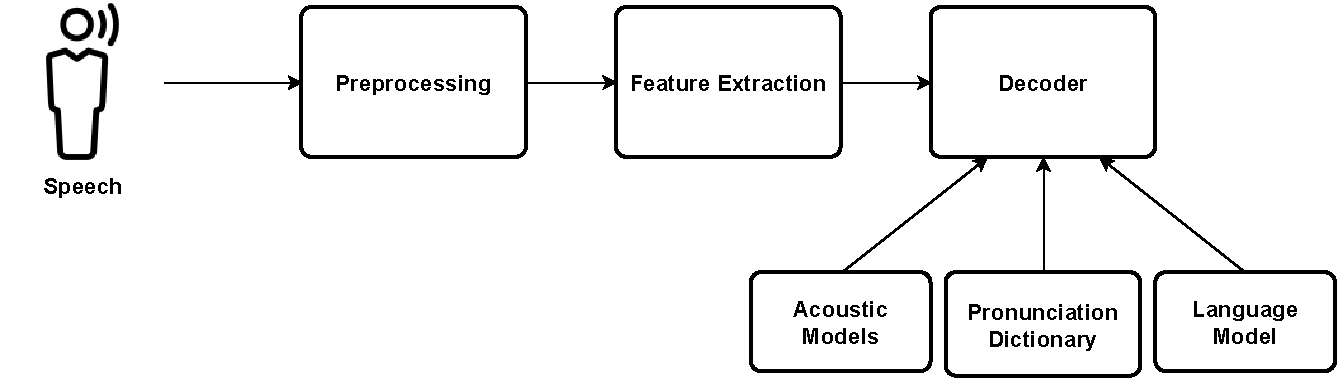
\includegraphics[width=\textwidth]{images/Tradition ASR System.pdf} 
    \caption{A traditional ASR system architecture}
    \label{fig:trad_asr_model}
  \end{center}
\end{figure}

In the above architecture, the speech signal is first preprocessed to remove any unwanted noise and then convert to the required format for the next steps. Next, feature extraction methods are applied to generate vectors which are used in the decoder. The decoder is composed of multiple models including acoustic models, pronunciation dictionary and language models. 

\subsection{End to end speech recognition systems}
\label{section:e2easr}
In end to end speech recognition systems, a single model, usually based on deep learning, supersedes the traditional ASR system stages. A deep learning model combined with an external language model can achieve higher performance than traditional speech pipelines, while being quite simple to train. These systems rely on large neural networks and are trained on multiple GPUs and thousands of hours of speech data. Since the system learns from the data directly, specialized components for capturing finer details of the speaker or other noise filtering components are not essential. On the contrary, previous experiments have shown that end to end models stand out in the cases where robustness is crucial. \cite{Hannun2014DeepRecognition}. 

\emph{In an end to end deep learning ASR system, we can achieve performance gains by improving three main components: model architecture, training data and computational infrastructure. The focus of this thesis is hence to increase the scale of data while making maximum use of the available computational resources, and trying out various experiments with different model architectures to analyse the effect it has on final performance of the system.}

\section{What are Deep Neural Networks?}
A deep neural network is a neural network with many hidden layers. Theoretically, deep neural networks can be trained to model non-linear models and functions for very high dimensional data. Traditionally, it was quite challenging to train deep neural networks, but there was a resurgence in the usage of deep neural networks in the previous decade, also in the field of speech recognition \cite{Dahl2012Context-DependentRecognition, Morgan2012DeepRecognition, DengRECENTMICROSOFT, Hannun2014DeepRecognition}. 

One of the first deep neural network was a Multilayer Perceptron (MLP), which consists of an input layer, an output layer and a hidden layer. This architecture is shown in Figure \ref{fig:mlp}. 

\begin{figure}[ht]
  \begin{center}
    % below the size of the figure has been reduced for example
    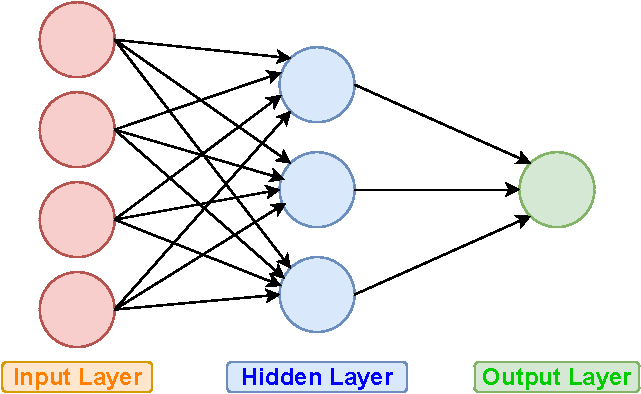
\includegraphics[width=\textwidth]{images/MLP.pdf} 
    \caption{An MLP architecture}
    \label{fig:mlp}
  \end{center}
\end{figure}

Each layer of this network consists of multiple neurons, and each of these neurons are associated with a weights matrix that determines how much a neuron should take part in the decision-making process. At each neuron, the input signal is multiplied with its corresponding weights and then added to have a weighed sum as the output of a layer. This can be represented as,

\[ z = w_1x_1 + w_2x_2 + .. + w_nx_n \]

In the above formula z is the weighted sum output, w is the weight, x is an input and there are n number of inputs. This weighted sum is then passed to an activation function like tanh, sigmoid, ReLU, etc. Each layer is computer at each step of training and the network is trained to increase the performance of the neural network. Error is computed after each training step, and then it is backpropogated to all the previous layers to improve the network weights. Backpropogation required an optimisation algorithm like Stochastic Gradient Descent (SGD), Adaptive Momentum Estimation (Adam), etc.

\subsection {Recurrent Neural Networks}
\subsection {Convolutional Neural Networks}
\subsection {Attention based CRDNN}


